\section{Physical Simulation}

\subsection{Dynamics Equations}

We model the robot as an articulated rigid body system in our simulator. We represent the states of the system $(\mathbf{x}, \dot{\mathbf{x}})$ in the generalized coordinate, where $\mathbf{x}$ include the global position $\mathbf{p}$, orientation $\mathbf{r}$ of the root link, and the joint angles $\mathbf{q}$. We solve the governing equations of motion eq.(\ref{eq:robotdynamics}) in the generalized coordinates.

\begin{equation}
\label{eq:robotdynamics}
\mathbf{M}(\mathbf{x})\mathbf{\ddot{x}}+\mathbf{C}(\mathbf{x},\mathbf{\dot{x}})=\mathbf{\tau}(\mathbf{q}, \dot{\mathbf{q}}, \bar{\mathbf{q}})+\mathbf{J}^T\mathbf{f}
\end{equation}
where $\mathbf{M}(\mathbf{x})$ is the mass matrix and $\mathbf{C}(\mathbf{x},\mathbf{\dot{x}})$ is the Coriolis and Centrifugal force. $\mathbf{\tau}(\mathbf{q}, \dot{\mathbf{q}}, \bar{\mathbf{q}})$ are joint torques exerted by the actuators, which depends on the current joint angles $\mathbf{q}$, velocities $\dot{\mathbf{q}}$ and desired angles $\bar{\mathbf{q}}$. $\mathbf{J}$ is the Jacobian matrix and $\mathbf{f}$ is the external contact force, which is computed based on linear complementarity conditions. In our implementation, we use DART to compute the contact force and numerically integrate the system state $(\mathbf{x}, \dot{\mathbf{x}})$ over time.

\subsection{Actuator Model}
\label{sec:motorDynamics}
Most of the actuators on our robot, BIOLOID GP, are ROBOTIS Dynamixel AX-18. The control signal for these actuators are desired angles $\bar{\mathbf{q}}$. Given the difference between the desired and the current angle ${q-\bar{q}}$ of each joint, the servo first maps it to a corresponding power level $U$, which is eventually converted to the joint torque $\tau$ according to the internal actuator dynamics. According to the specification of the servo, we derive the relation between the output torque $\tau$, the current joint state $q, \dot{q}$ and the desired angle $\bar{q}$. The detailed derivation of this relation is shown in Appendix.

\begin{equation}
  \tau = -k_p(q-\bar{q}) - k_d\dot{q} - k_c\sgn(\dot{q})\\
    \label{eqn:torqueErrorRelationSimple}
\end{equation}

We call these values $k_p$, $k_d$ and $k_c$ the \emph{actuator gains}. Note that despite the similarity, they are not PID gains. Dynamixel AX-18 servos do not have the capabilities to tune PID gains. These gains are determined by the design of the servo, which are unknown for us.

We design robot experiments to identify the actuator gains $k_p$, $k_d$ and $k_c$. In the experiment, we clamp the entire robot on a table except for the left foot. We then send a periodic control signal $\bar{q}(t)$ to the servo at the left ankel (blue curve in Figure \ref{fig:actuatorId} Left). The desired joint angle stays at the maximum value for 0.67 second, then changes to the minimum value and stays for another 0.67 second and repeats. We record the trajectory of the actual joint angle $q(t)$ through the experiment (green curve in Figure \ref{fig:actuatorId} Left). The black ``+'' in Figure~\ref{fig:actuatorId} Right shows the error $\Delta q = q-\bar{q}$ in a small segment of time.

\begin{figure}[!t]
  \centering
  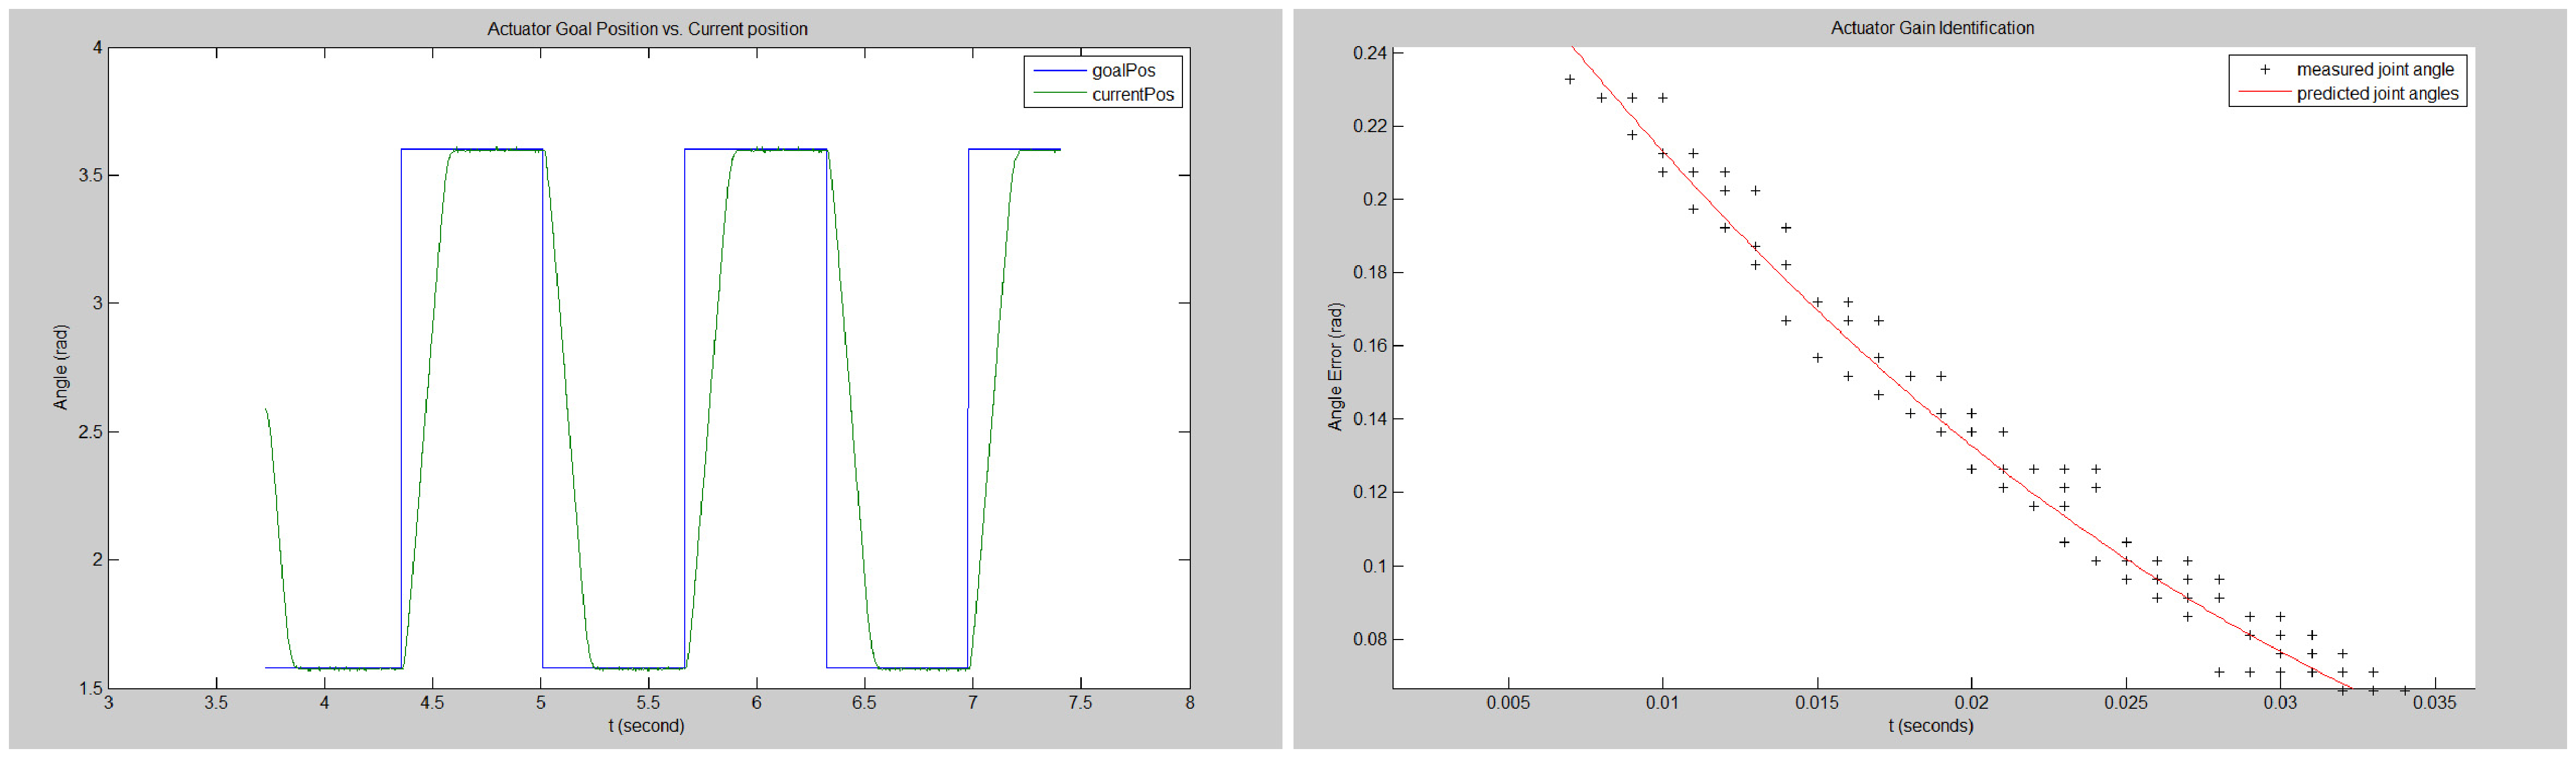
\includegraphics[width=0.5\textwidth]{figures/actuatorId}
  \caption{Actuator Identification. Left: the time series of input desired joint angle and the measured joint angle for an AX-18 servo. Right: the time series of actual error of joint angle and the predicted error using the identified actuator gains.  }
  \label{fig:actuatorId}
\end{figure}

Given $q(t)$ and $\bar{q}(t)$, we can apply regression to estimate the actuator gains. From eq. (\ref{eqn:torqueErrorRelationSimple}), we have
\begin{equation}
\ddot{q}=I^{-1}(-k_p\Delta q - k_d\dot{q} - k_c\sgn(\dot{q}))
\end{equation}
where $I$ is the moment of inertia of the foot with respect to the rotating axis. The above equation is derived by plugging into $\tau = I\ddot{q}+\dot{I}\dot{q}$ and the fact that $\dot{I}\dot{q}=0$ because the foot is a rigid body that rotates along a fixed axis. Ideally, $\ddot{q}$ and $\dot{q}$ can be computed using finite difference. However, the measurement of $q(t)$ is too noisy and finite difference would greatly magnify the noise. To solve this problem, we first smooth $q(t)$ by performing a 4th-order polynomial regression:
\begin{equation}
  \min_{a,b,c,d,e}\int ||q(t)-(at^4+bt^3+ct^2+dt+e)||^2\mathrm{d}t
  \label{eqn:Deltaq}
\end{equation}
where $a,b,c,d,e$ are the polynomial coefficients. This regression gives us a smooth analytical expression of $q(t)$. We then compute $\ddot{q}$ and $\dot{q}$ by differentiate this polynomial analytically:
\begin{align}
\label{eqn:Deltaqdot}  \dot{q}(t)&=4at^3+3bt^2+2ct+d\\
\label{eqn:Deltaqddot}  \ddot{q}(t)&=12at^2+6bt+2c
\end{align}

Combining eq. (\ref{eqn:Deltaq}), (\ref{eqn:Deltaqdot}) and (\ref{eqn:Deltaqddot}), we can perform another regression to compute the actuator gains.
\begin{equation}
\min_{k_p, k_d, k_c}\int||\ddot{q}(t)-I^{-1}(-k_p(q(t)-\bar{q}(t)) - k_d\dot{q}(t) - k_c\sgn(\dot{q}(t)))||^2\mathrm{d}t
\end{equation}

Our experiments and computation show that the actuator gains are $k_p=9.272(N\cdot m/rad)$, $k_d=0.3069(N\cdot m\cdot s/rad)$, and $k_c=0.03(N\cdot m)$. To verify the correctness of these values, we plug them into the simulator and repeat the same experiment in the simulation. The red curve in Figure \ref{fig:actuatorId} Right is the error over time predicted in our simulation, which agrees well with the data that was collected from the robot experiment.


